\chapter{Implementation}

% \epigraph{The best presents don't come in boxes.}{Bill Watterson}

\begin{figure}[H]
	\centering
	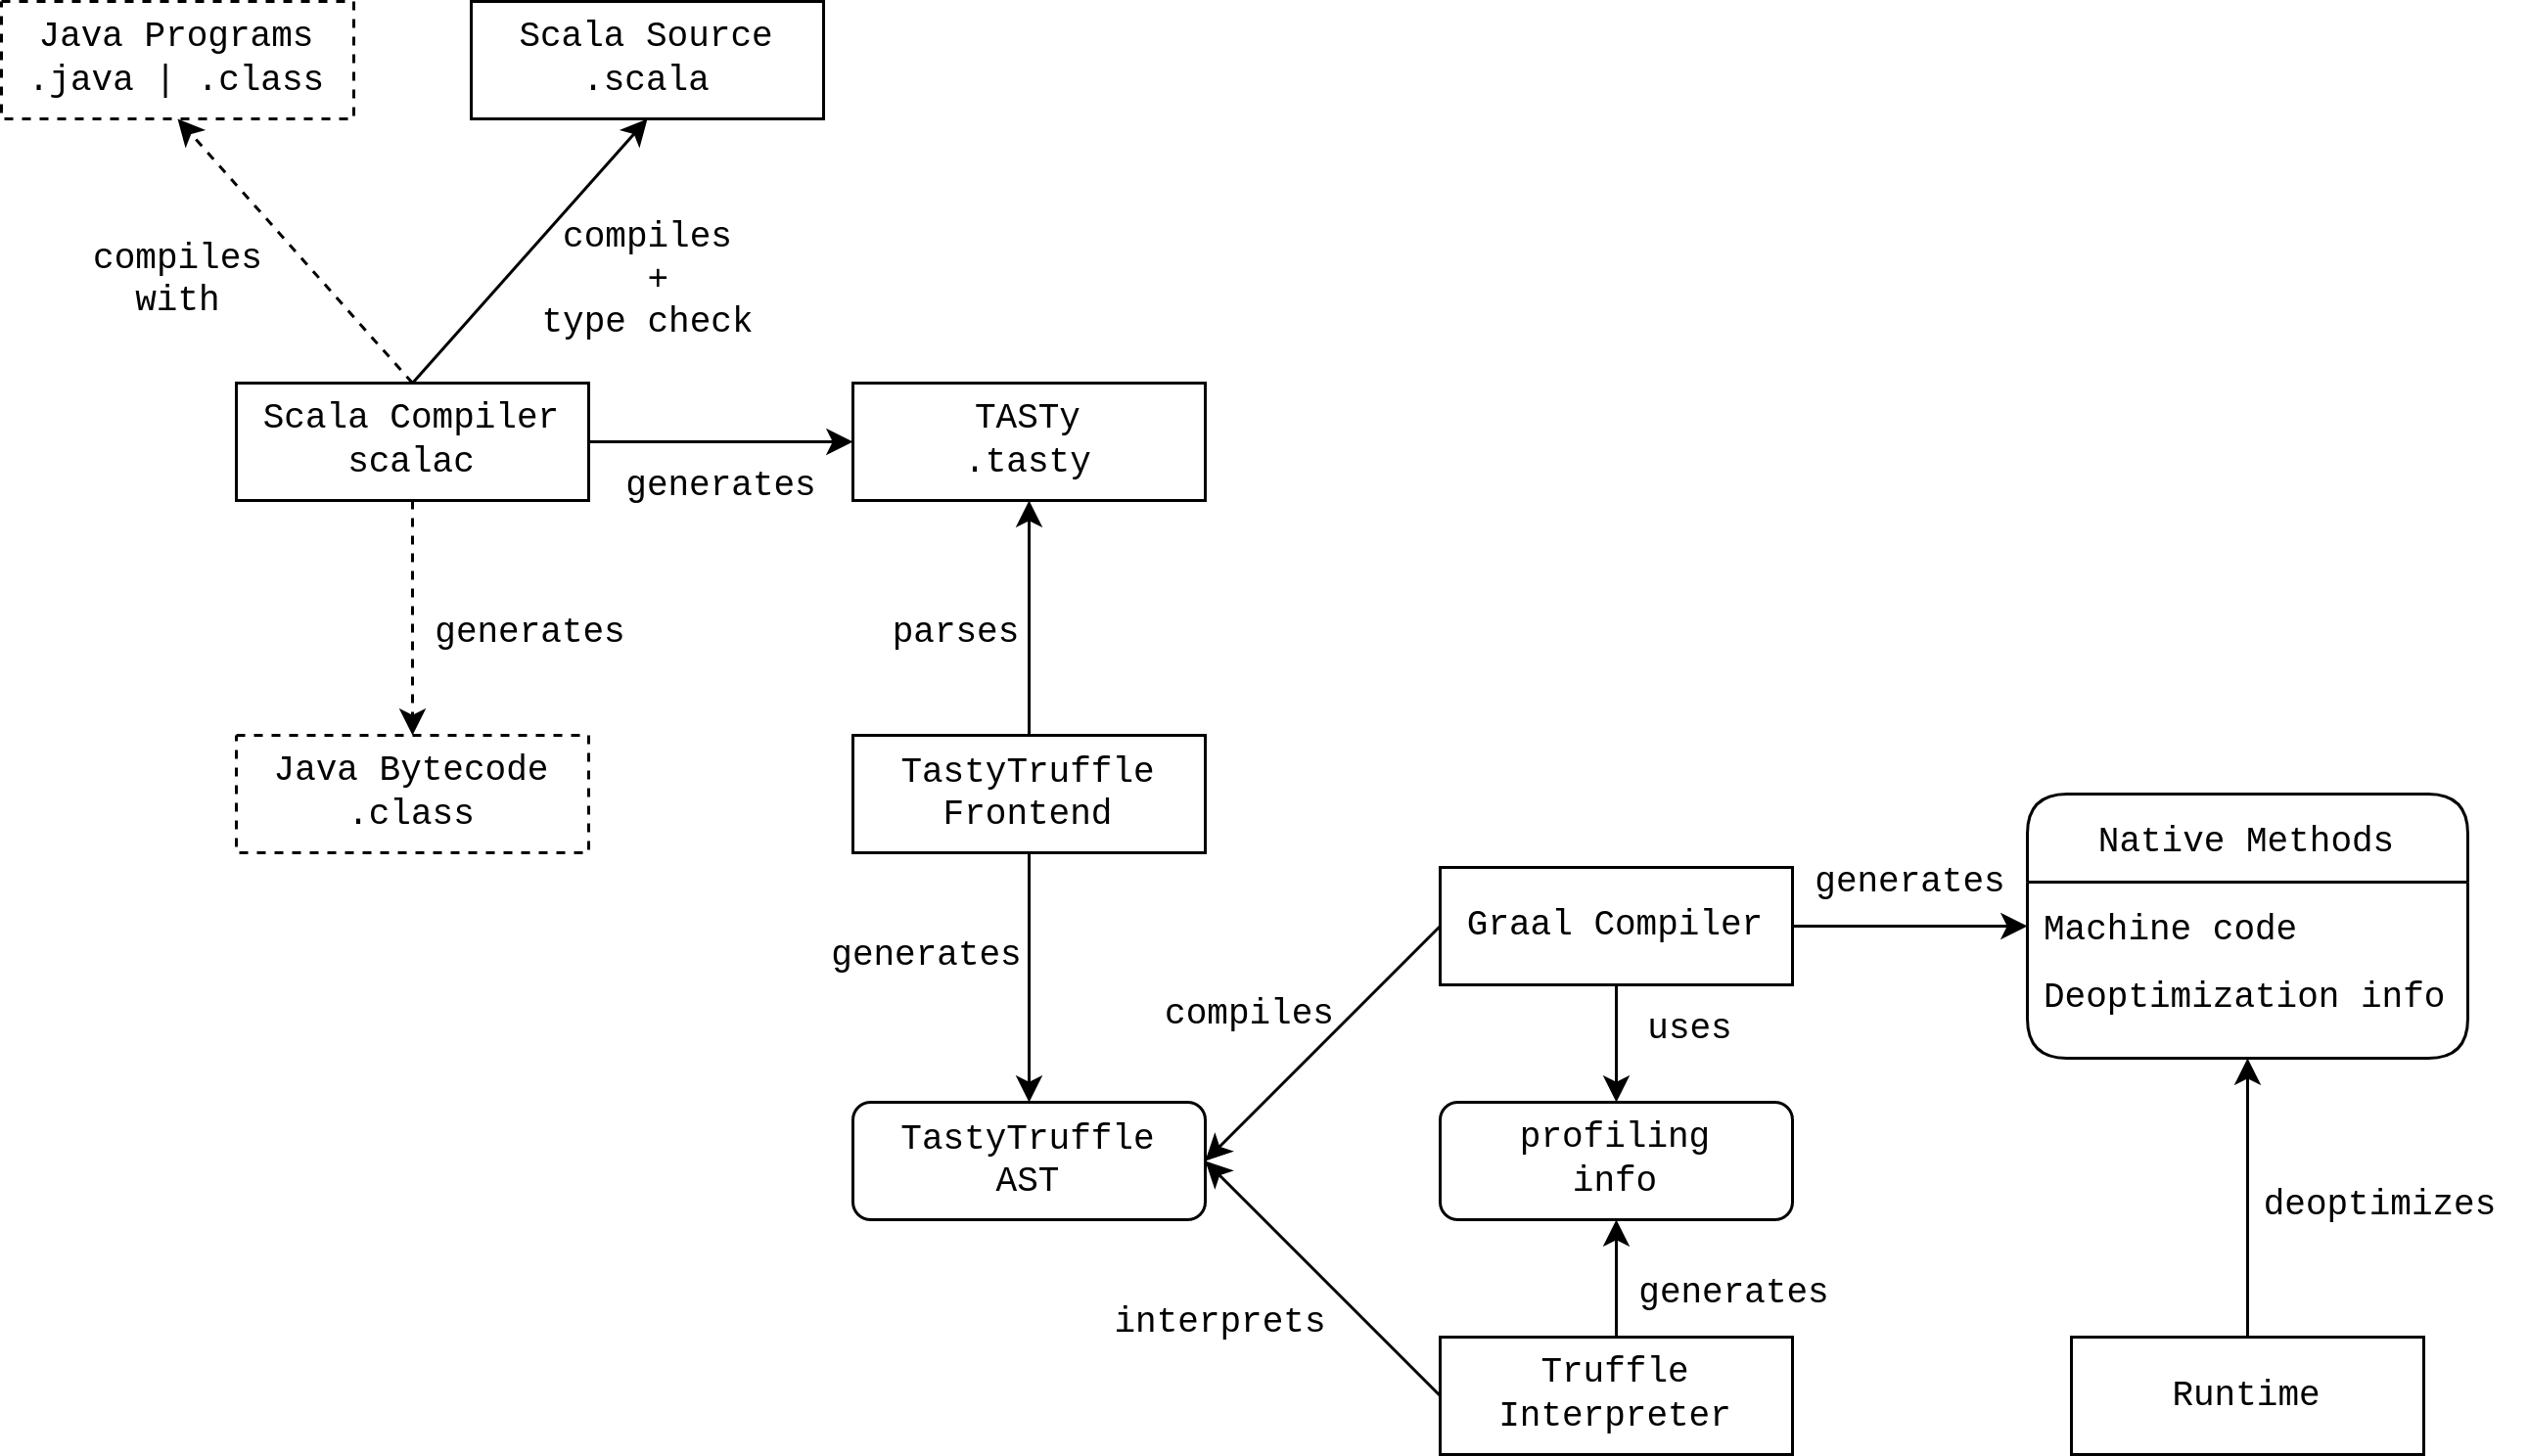
\includegraphics[width=0.5\textwidth]{figures/tastytruffle-pipeline.png}
	\caption{TastyTruffle in the context of the Scala compilation pipeline.}
\end{figure}

\section{Case Study: A List in TastyTruffle}

\begin{figure}[H]
	\begin{minted}{scala}
		abstract class List[+T] {
			def head: T
			def tail: List[T]
			def length: Int
			def isEmpty: Boolean = length == 0
			def contains[T1 >: T](elem: T1): Boolean
		}
	\end{minted}
	\caption{Definition of an abstract \texttt{List} class}
\end{figure}

\begin{figure}[H]
	\begin{minted}{scala}
		case class ::[+T](head: T, tail: List[T]) extends List[T] {
			override def length: Int = 1 + tail.length
			
			override def contains[T1 >: T](elem: T1): Boolean = {
				var these: List[T] = this
				while (!these.isEmpty) 
					if (these.head == elem) return true
					else these = these.tail
				false
			}
			
			override def hashCode(): Int = {
				var these: List[T] = this
				var hashCode: Int = 0
				while (!these.isEmpty) {
					val headHash = these.head.hashCode()
					if (these.tail.isEmpty) hashCode = hashCode | headHash
					else hashCode = hashCode | headHash >> 8
					these = these.tail
				}
				hashCode
			}
		}
		
		case object Nil extends List[Nothing] {
			override def head: Nothing = throw new NoSuchElementException("head of empty list")
			override def tail: Nothing = throw new UnsupportedOperationException("tail of empty list")
			override def length: Int = 0
			override def contains[T1 >: Nothing](elem: T1): Boolean = false
			override def hashCode(): Int = 0
		}
	\end{minted}
	\caption{Implementations of \texttt{List} class}
\end{figure}

\section{TastyTruffle Intermediate Representation}

Scala programs in \acrshort{tasty} format are unsuitable for execution in a Truffle interpreter. Programs in must be parsed and transformed into an executable representation in \textsc{TastyTruffle}. As TASTy represents a Scala program close to its equivalent source representation, canonicalization compiler passes (see appendix \ref{appendix:dotty-phases}) that would otherwise normalize the IR are not present. Instead, we implement TastyTruffle IR to represent a canonicalized executable intermediate representation which can be specialized on demand. 


The following sections will introduce the nodes in TastyTruffle IR and how they are derived from Scala source and TASTy.

% TODO: insert TASTy tree diagrams.

\subsection*{Local Variables and Values} 

There are two distinct methods for declaring local variables in Scala:

\begin{figure}[H]
	\begin{minted}{scala}
		// Constant reference, cannot be reassigned.
		val constant: Int = 0 
		var variable: Int = 1
		...
		variable = 2
	\end{minted} 
	\caption{\scalainline{val} and \scalainline{var} variable declarations}
\end{figure}

As the \mintinline{scala}|val| abstraction is syntactic sugar\cite{mechanical-eval-of-exprs} for the Scala compiler to validate that a \scalainline{val} definition is never reassigned, 
\textsc{TastyTruffle} does not distinguish between \scalainline{val} and \scalainline{var} variable declarations. Each unique variable declaration 
has a corresponding frame slot in the frame descriptor of its root node. While Scala has lexical scoping\cite{scala:lang-spec}, scope resolution occurs after pickling at a later stage in Scala compilation.
As a result, symbols do not contain sufficient information to disambiguate between scopes. We consider variable declarations which share the same symbol but not the same \texttt{Block} trees 
to be unique in order to address this.

Truffle permits each frame slot in a frame descriptor be described by a \textit{frame slot kind}. At the time of writing, a frame slot kind is given as:

\begin{figure}[H]
	\begin{minted}{scala}
		object FrameSlotKind extends Enumeration {
			type FrameSlotKind = Value
			val Object, Long, Int, Double, Float, Boolean, Byte = Value
		}
	\end{minted}
	\caption{Simplified implementation of \scalainline{FrameSlotKind}}
\end{figure}

We determine the frame slot kind of a type using the following method:

\begin{figure}[H]
	\begin{minted}{scala}
	def getFrameSlotKind(tpe: Type): Option[FrameSlotKind] = {
		if (tpe.isMonomorphic && tpe.isPrimitive)
			Some(primitiveSlotKindOf(tpe))
		else if (tpe.isParameter)
			None
		else
			Some(FrameSlotKind.Object)
	}	
	\end{minted}
	\caption{Pseudocode for determining the frame slot kind of a type.}
\end{figure}

Truffle specializes local variable access based on the variable's type during partial evaluation\cite{truffle:pe}. To simplify and eliminate the need to specialize read and writes of variables where types are monomorphic and statically refer to a primitive type, the primitive frame slot kind is matched in the frame descriptor. In all other cases, including when the type is not resolvable through a single type parameter, e.g. \scalainline{val x: T}, we assign the frame slot the \scalainline{Object} frame slot kind. We will defer discussion of variable declarations which have polymorphic types that cannot be resolved statically until section \ref{implementation:specialization}.

\subsection*{Terms}

\subsubsection*{Binary Expressions}

\subsubsection*{Member Access}

\subsubsection*{Control Structures}

\subsubsection*{Calls}

\begin{figure}[H]
	\begin{minted}{scala}
	class ApplyNode(sig: Signature, receiver: TermNode, args: Array[TermNode]) extends TermNode {
		
		final val INLINE_CACHE_SIZE: Int = 5;
		
		@Specialization(guards = "inst.type == tpe", limit = "INLINE_CACHE_SIZE")
		def cached(
			frame: VirtualFrame,
			inst: ClassInstance,
			@Cached("inst.type") tpe: Type,
			@Cached("create(resolveCall(instance, sig)") callNode: DirectCallNode
		): Object = callNode.call(evalArgs(frame, inst));
		
		@Specialization(replaces = "cached")
		def virtual(
			frame: VirtualFrame,
			inst: ClassInstance,
			@Cached callNode: IndirectCallNode
		): Object = {
			val callTarget = resolveCall(instance, sig);
			callNode.call(callTarget, evalArgs(frame, inst))
		}
	}
	\end{minted}
	\caption{Simplified implementation of the call node used in TastyTruffle.}
	
\end{figure}

	
\begin{figure}[H]
	\centering
	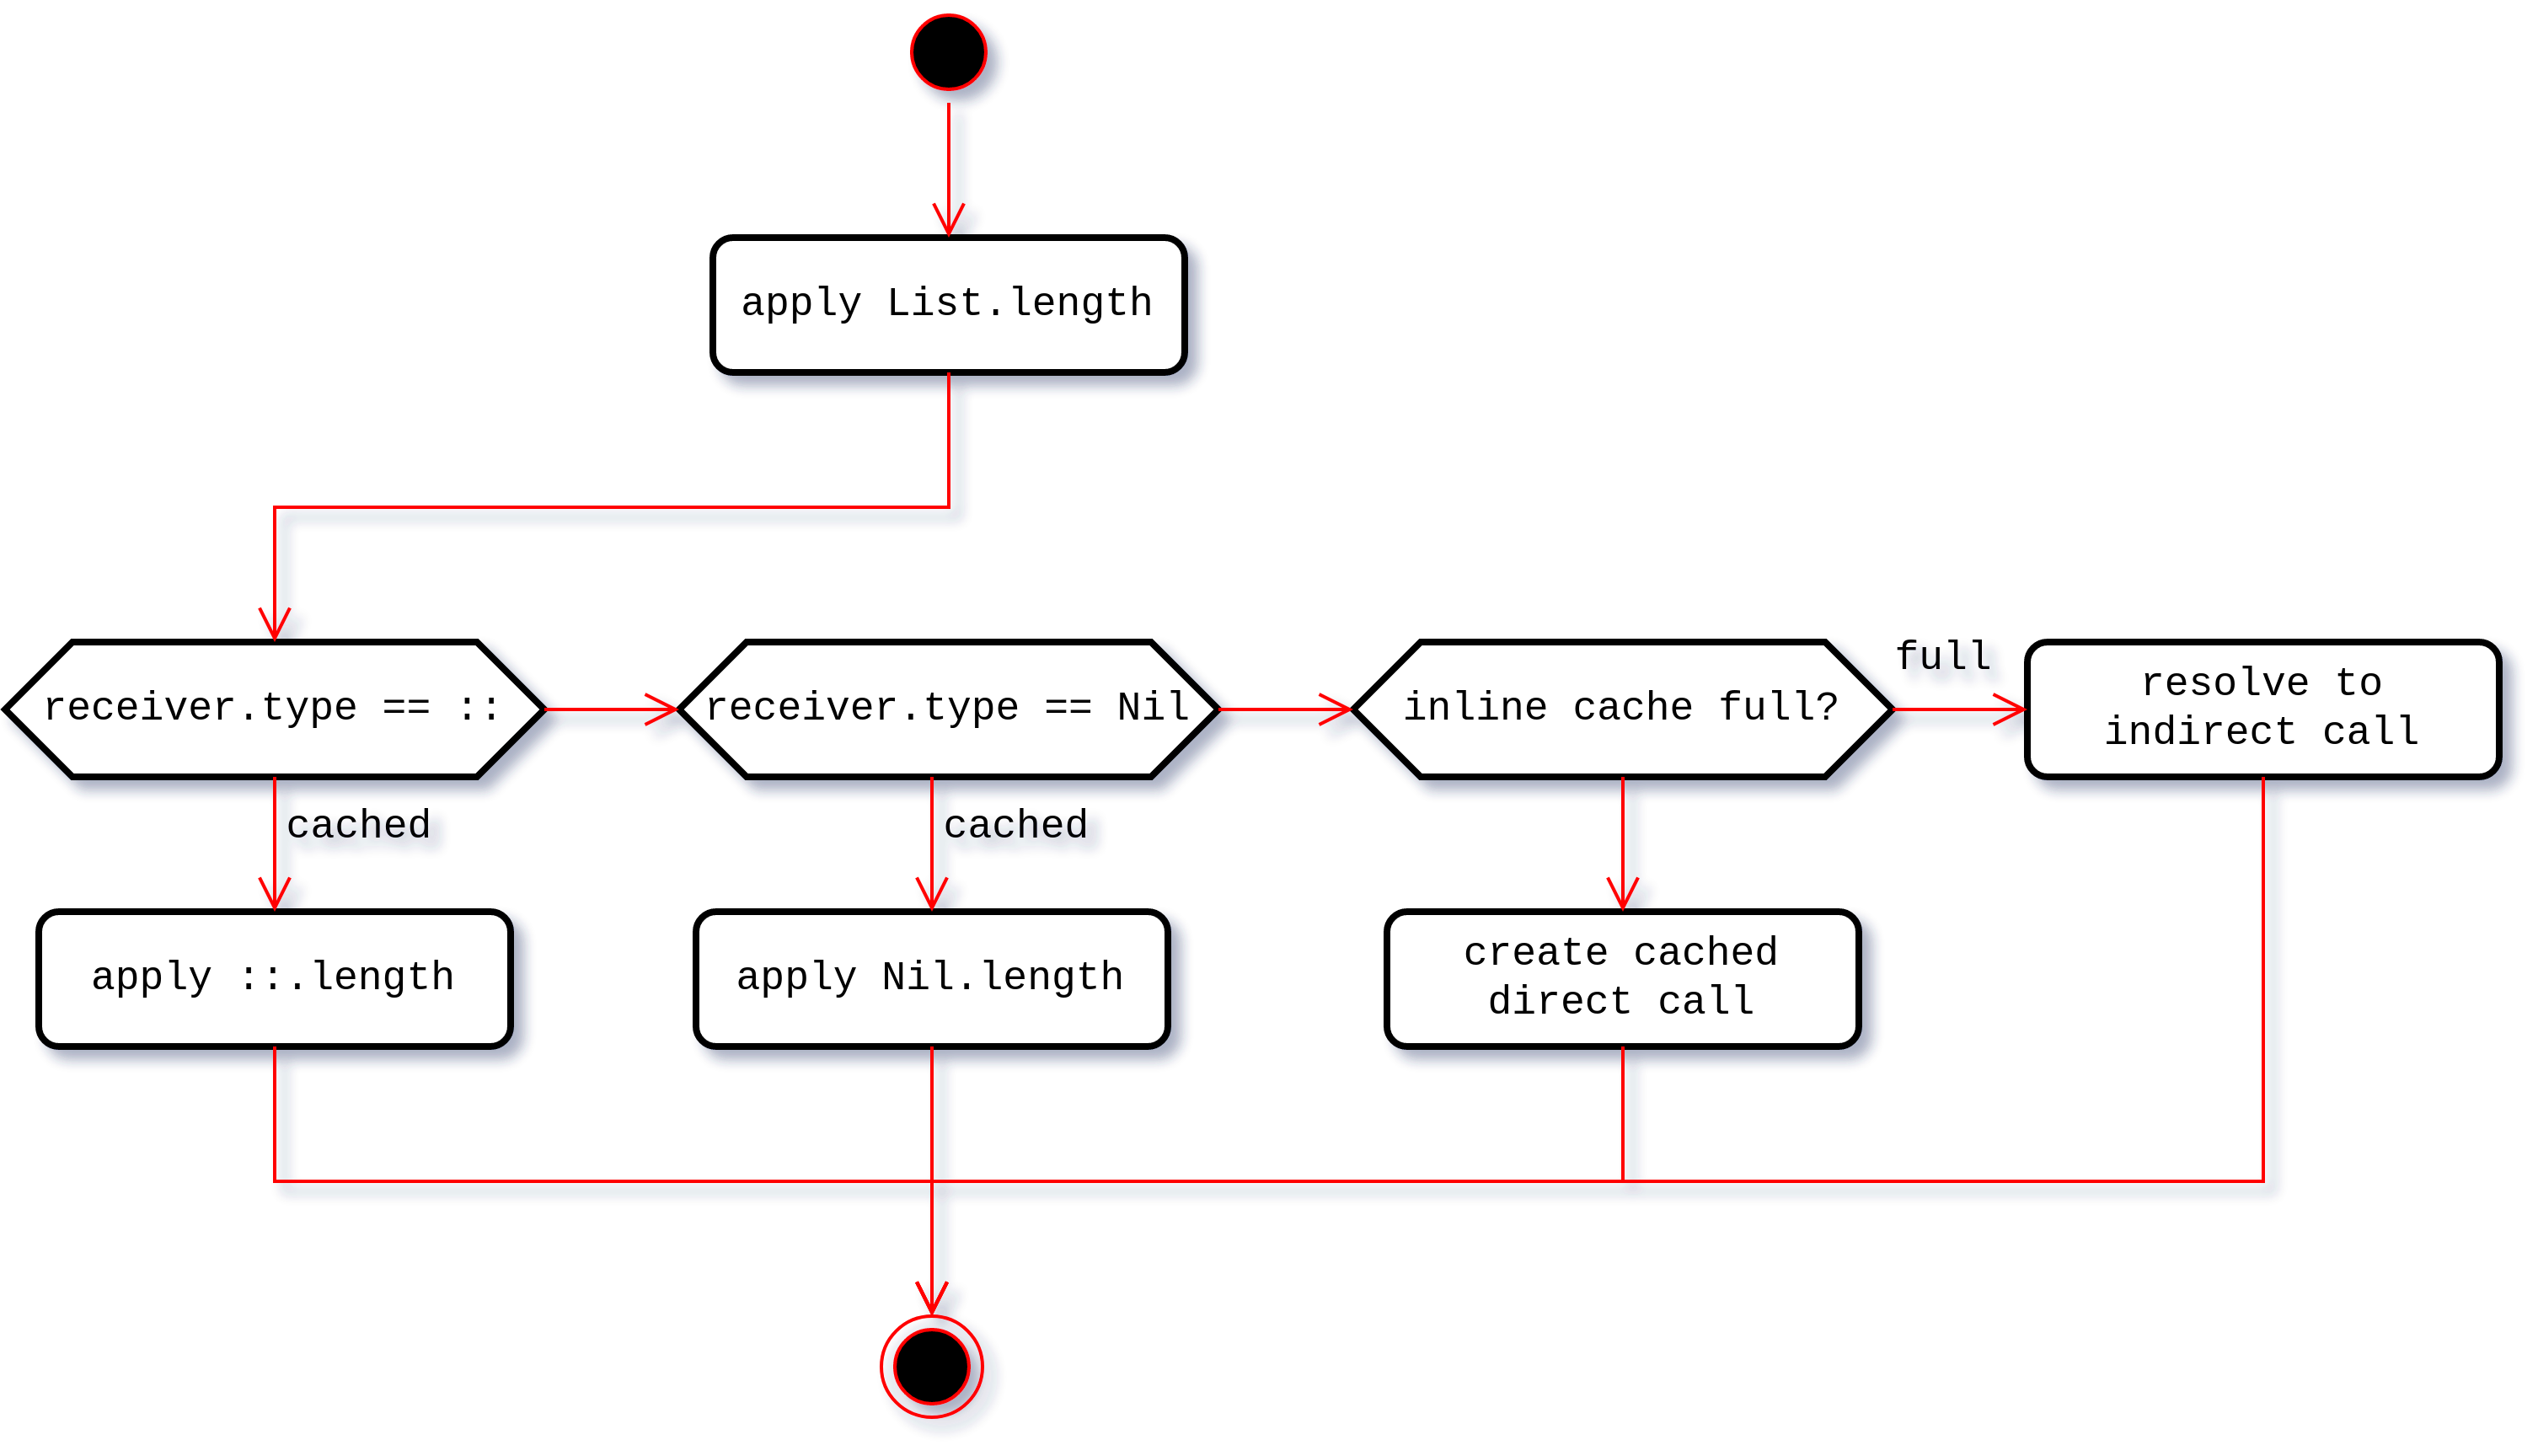
\includegraphics[width=0.5\textwidth]{figures/tastytruffle-indirect-example.png}
	\caption{A flow diagram for the virtual dispatch of \scalainline{List.length}}
\end{figure}

\subsection*{Object Allocation}

\subsection*{Types}

\section{Specialization}
\label{implementation:specialization}

\begin{figure}[H]
	\begin{minted}{scala}
		trait PolymorphicTermNode extends TermNode {
			def resolveType: ClassType 
			override def execute(frame: VirtualFrame): Object = 
				throw new UnsupportOperationException("generic code cannot be executed!")
		}
	\end{minted}
	\caption{A placeholder node for polymorphic code in \textsc{TastyTruffle}}
\end{figure}

\subsection{Specializing Terms}

The basic polymorphic unit of code in Scala are terms whose types are derived directly from a type parameter \mintinline{scala}|T| or indirectly from a type constructor such as \mintinline{scala}|Array[T]|. Polymorphic terms can be divided into the following categories:

\subsubsection*{Polymorphic local access}
\subsubsection*{Polymorphic field access}
\subsubsection*{Polymorphic method call}
\subsubsection*{Polymorphic instantiation}


\subsection{Specializing Methods}

Generic methods in Scala can be polymorphic under class type parameters, method type parameters, or both. In the latter two cases, polymorphic methods contain additional reified type parameters. In addition to the polymorphic terms present in the method body discussed in the previous section, the type of method term parameters may be polymorphic. The following components of a generic method must specialized:

\begin{itemize}
	\item Polymorphic method parameters.
	\item Polymorphic terms inside the method body.
\end{itemize}


\subsubsection*{Method Parameters}

\subsubsection*{Typed Dispatch}

\begin{figure}[H]
	\begin{minted}{scala}
	class TypeDispatchNode(parent: RootNode) extends TermNode {
		
		type TypeArguments: Array[Type]
		@CompilerDirectives.CompilationFinal
		var cache: Map[TypeArguments, DirectCallNode]
		
		override def execute(frame: VirtualFrame): Object = {
			val types: TypeArguments = resolveTypeParameters(frame)
			dispatch(frame, args);
		}
		
		def dispatch(frame: VirtualFrame, types: TypeArguments): Object = cache.get(types) match {
			case Some(callNode) => callNode.call(frame.getArguments)
			case None => createAndDispatch(frame, types)
		}
		
		def createAndDispatch(frame: VirtualFrame, types: TypeArguments): Object = {
			CompilerDirectives.transferToInterpreterAndInvalidate()
			val specialization = parent.specialize(types)
			val callNode = DirectCallNode.create(specialization)
			cache = cache.updated(types, callNode)
			callNode.call(frame.getArguments)
		}
	}
	\end{minted}
\caption{Simplified implementation of generic dispatch node based on reified type arguments.}
\end{figure}

\subsubsection*{Code Duplication}

\subsubsection*{Partial Evaluation}

\section{Specializing Classes}
